%!Tex Root=**/main.tex
\mode<article>{\chapter{3D Gaussian Splatting}}
\mode<presentation>{\section{3D Gaussian Splatting}}

\mode<article>{\section{3D Gaussian Splatting}}
\mode<presentation>{\subsection{3D Gaussian Splatting}}

\begin{frame}<all>[c]
	\mode<presentation>{\Frametitle{Framework}}
	\begin{figure}[htbp]
		\centering
		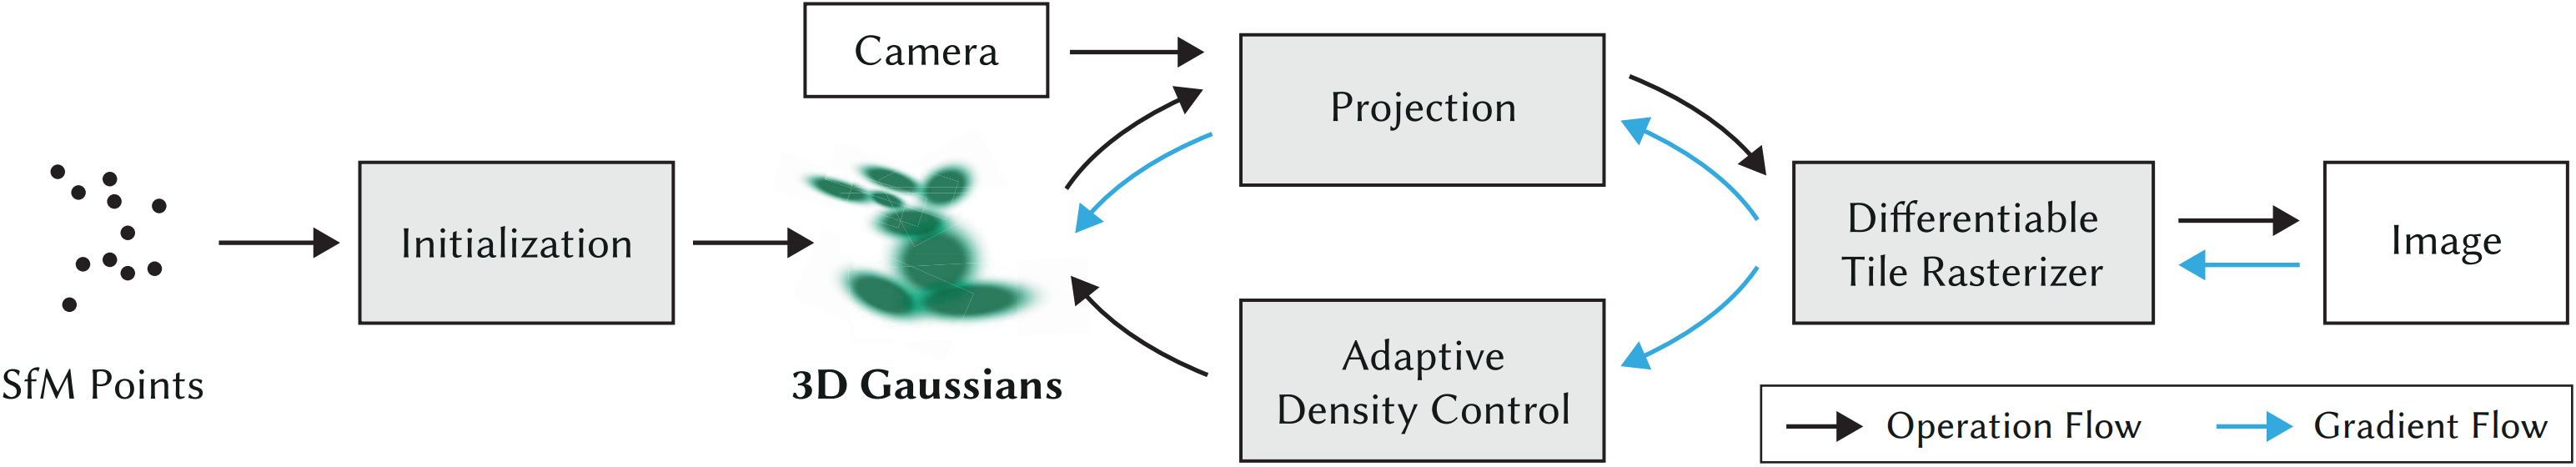
\includegraphics[width=\linewidth]{3dgs-overview.png}
		\smallskip
		\caption{Overview of 3DGS~\autocite{kerbl3Dgaussians}}
	\end{figure}
	\mode<presentation>{\blfootnote{\href{https://repo-sam.inria.fr/fungraph/3d-gaussian-splatting/}{(SIGGRAPH 2023, Best Paper) 3D gaussian splatting for real-time radiance field rendering}}}
\end{frame}

\mode<article>{\subsection{Rendering Pipeline}\label{sec:3dgs-rendering-pipeline}}
\mode<article>{\subsubsection{3D Representation}}
\begin{frame}<all>[c]
	\mode<presentation>{\Frametitle{3D Representation}}
	\mode<article>{
		\par \alert<all>{Optimizable} and \alert<all>{point-based} 3D Gaussians inherent the best of two worlds.
	}
	\begin{block}{3D Gaussian Primitives}
		\resetcolorseries[6]{marknode-color-series}
		\resetcolorseries[6]{annotation-color-series}
		\begin{equation}
			\label{eq:3dgs-representation}
			\tikzmarknode{n0}{\colorbox{marknode-color-series!![0]}{\(\mathcal{S}\)}}  = \left\{ \mathcal{G}_i \vert i = 0,1,\cdots,N \right\}
			,\text{ where }
			\mathcal{G}_i = \left\{
			\tikzmarknode{n1}{\colorbox{marknode-color-series!![1]}{\(\mathbf{p}\)}},
			\tikzmarknode{n2}{\colorbox{marknode-color-series!![2]}{\(\mathbf{q}\)}},
			\tikzmarknode{n3}{\colorbox{marknode-color-series!![3]}{\(\mathbf{s}\)}},
			\tikzmarknode{n4}{\colorbox{marknode-color-series!![4]}{\(\mathbf{c}\)}},
			\tikzmarknode{n5}{\colorbox{marknode-color-series!![5]}{\(\alpha\)}}
			\right\}
		\end{equation}
		\begin{annotatedEquationEnv}
			\annotatedEquation{colorseries}{n0}{south}{0em}{-1em}{north west}{annotation-color-series}{scene}{east}
			\annotatedEquation{colorseries}{n1}{south}{0em}{-1em}{north east}{annotation-color-series}{\(\in \mathbb{R}^3\), position (mean)}{west}
			\annotatedEquation{colorseries}{n2}{south}{0em}{-2.5em}{north east}{annotation-color-series}{\(\in \mathrm{SO}(3)\), rotation (component of covariance)}{west}
			\annotatedEquation{colorseries}{n3}{south}{0em}{-4em}{north east}{annotation-color-series}{\(\in \mathbb{R}^3\), scale (component of covariance)}{west}
			\annotatedEquation{colorseries}{n4}{south}{0em}{-5.5em}{north east}{annotation-color-series}{\(\in \mathbb{R}^{3n}\), color (spherical harmonics)}{west}
			\annotatedEquation{colorseries}{n5}{south}{0em}{-7em}{north east}{annotation-color-series}{\(\in (0,1] \), opacity}{west}
		\end{annotatedEquationEnv}
		\vspace*{7em}
	\end{block}
	\mode<presentation>{\blfootnote{\href{https://repo-sam.inria.fr/fungraph/3d-gaussian-splatting/}{(SIGGRAPH 2023, Best Paper) 3D gaussian splatting for real-time radiance field rendering}}}
	\mode<presentation>{\blfootnote{\href{http://arxiv.org/abs/2404.19706}{(SIGGRAPH 2024) RTG-SLAM: Real-time 3D Reconstruction at Scale using Gaussian Splatting}}}
\end{frame}

\mode<article>{\subsubsection{Splatting}}
\begin{frame}<all>[c]
	\mode<presentation>{\Frametitle{Splatting}}
	\par ``3D ellipsoids'' are splatted to ``2D ellipses''.
	\begin{block}{Splatting}
		\begin{minipage}[c]{0.45\linewidth}
			\resetcolorseries[4]{marknode-color-series}
			\resetcolorseries[4]{annotation-color-series}
			\begin{equation}\label{eq:3dgs-projection-mean}
				\tikzmarknode{n3}{\colorbox{marknode-color-series!![3]}{\(\mu_{i}\)}}
				=
				\tikzmarknode{n2}{\colorbox{marknode-color-series!![2]}{\(\pi\)}}
				\left(
				\tikzmarknode{n1}{\colorbox{marknode-color-series!![1]}{\(\mathbf{T}_{cw}\)}}
				\cdot
				\tikzmarknode{n0}{\colorbox{marknode-color-series!![0]}{\(\mu_{w}\)}}
				\right)
			\end{equation}
			\begin{annotatedEquationEnv}
				\annotatedEquation{colorseries}{n0}{south}{0em}{-1em}{north west}{annotation-color-series}{\(\in \mathbb{P}^3\), 3D(world) mean}{east}
				\annotatedEquation{colorseries}{n1}{south}{0em}{-3em}{north west}{annotation-color-series}{\(\in \mathrm{SE}(3)\), camera pose}{east}
				\annotatedEquation{colorseries}{n2}{south}{0em}{-5em}{north west}{annotation-color-series}{projection}{east}
				\annotatedEquation{colorseries}{n3}{south}{0}{-7em}{north west}{annotation-color-series}{\(\in \mathbb{P}^2\), 2D(image) mean}{east}
			\end{annotatedEquationEnv}
		\end{minipage}
		\begin{minipage}[c]{0.50\linewidth}
			\resetcolorseries[4]{marknode-color-series}
			\resetcolorseries[4]{annotation-color-series}
			\begin{equation}\label{eq:3dgs-projection-covariance}
				\tikzmarknode{n3}{\colorbox{marknode-color-series!![3]}{\(\Sigma_{i}\)}}
				=
				\tikzmarknode{n2}{\colorbox{marknode-color-series!![2]}{\(\mathbf{J}_{\pi}\)}}
				\tikzmarknode{n1}{\colorbox{marknode-color-series!![1]}{\(\mathbf{R}_{cw}\)}}
				\tikzmarknode{n0}{\colorbox{marknode-color-series!![0]}{\(\Sigma_{w}\)}}
				\mathbf{R}_{cw}^{\mathrm{T}} \mathbf{J}_{\pi}^{\mathrm{T}}
			\end{equation}
			\begin{annotatedEquationEnv}
				\annotatedEquation{colorseries}{n0}{south}{0em}{-1em}{north west}{annotation-color-series}{\(\in \mathbb{R}^{3\times 3}\),\\3D(world) covariance}{east}
				\annotatedEquation{colorseries}{n1}{south}{0em}{-3.5em}{north west}{annotation-color-series}{\(\in \mathrm{SO(3)}\),\\rotation component of \(\mathbf{T}_{cw}\)}{east}
				\annotatedEquation{colorseries}{n2}{south}{0em}{-6em}{north west}{annotation-color-series}{\(\in \mathbb{R}^{2\times 3}\), Jacobian of the \\linear approximation of \(\pi\)}{east}
				\annotatedEquation{colorseries}{n3}{south}{0em}{-8.5em}{north west}{annotation-color-series}{\(\in \mathbb{R}^{2\times 2}\), 2D(image) covariance}{east}
			\end{annotatedEquationEnv}
		\end{minipage}
		\vspace*{8.5em}
	\end{block}
	\mode<presentation>{\blfootnote{\href{https://repo-sam.inria.fr/fungraph/3d-gaussian-splatting/}{(SIGGRAPH 2023, Best Paper) 3D gaussian splatting for real-time radiance field rendering}}}
\end{frame}

\mode<article>{\subsubsection{Projection}}
\begin{frame}<all>[c]
	\mode<presentation>{\Frametitle{Projection}}
	\begin{block}{Projection}
		\resetcolorseries[7]{marknode-color-series}
		\resetcolorseries[7]{annotation-color-series}
		\vspace*{2em}
		\begin{equation}
			\tikzmarknode{n0}{\colorbox{marknode-color-series!![0]}{\(\mathbf{r}\)}}
			\left(
			\tikzmarknode{n1}{\colorbox{marknode-color-series!![1]}{\(\mathbf{u}\)}}
			\right) =
			\left(
			\tikzmarknode{n2}{\colorbox{marknode-color-series!![2]}{\(\mathbf{R}\)}}
			\tikzmarknode{n3}{\colorbox{marknode-color-series!![3]}{\(\mathbf{K}\)}}^{-1}
			\tikzmarknode{n4}{\colorbox{marknode-color-series!![4]}{\(\dot{\mathbf{u}}\)}}
			\right)
			\tikzmarknode{n5}{\colorbox{marknode-color-series!![5]}{\(\theta\)}}
			+
			\tikzmarknode{n6}{\colorbox{marknode-color-series!![6]}{\(\mathbf{t}\)}}
		\end{equation}
		\begin{annotatedEquationEnv}
			\annotatedEquation{colorseries}{n0}{south}{0em}{-0.5em}{north east}{annotation-color-series}{ray through pixel \(\mathbf{u}\)\\and optical center}{west}
			\annotatedEquation{colorseries}{n1}{south}{0em}{-3em}{north east}{annotation-color-series}{\(= \begin{bmatrix}
				h & w
			\end{bmatrix}^{\mathrm{T}}\), pixel}{west}
			\annotatedEquation{colorseries}{n2}{south}{0em}{-4em}{north west}{annotation-color-series}{\(\in \mathrm{SO(3)}\), rotation component of camera's pose \(\mathbf{T}\)}{east}
			\annotatedEquation{colorseries}{n3}{south}{0em}{-2.5em}{north west}{annotation-color-series}{camera's intrinsic matrix}{east}
			\annotatedEquation{colorseries}{n4}{south}{0em}{-1em}{north west}{annotation-color-series}{\(=\begin{bmatrix}
					h & w & 1
				\end{bmatrix}\), homogenous representation of \(\mathbf{u}\)}{east}
			\annotatedEquation{colorseries}{n5}{north}{0em}{1em}{south east}{annotation-color-series}{\(\in \mathbb{R}\), length parameter}{west}
			\annotatedEquation{colorseries}{n6}{north}{0em}{1em}{south west}{annotation-color-series}{\(\in \mathbb{R}^3\),\\translation component of camera's pose \(\mathbf{T}\)}{east}
		\end{annotatedEquationEnv}
		\vspace*{4em}
	\end{block}
	\mode<presentation>{\blfootnote{\href{https://repo-sam.inria.fr/fungraph/3d-gaussian-splatting/}{(SIGGRAPH 2023, Best Paper) 3D gaussian splatting for real-time radiance field rendering}}}
\end{frame}

\mode<article>{\subsubsection{\(\boldsymbol\alpha\)-blending}}
\begin{frame}<all>[c]
	\mode<presentation>{\Frametitle{\(\boldsymbol\alpha\)-blending}}
	\begin{block}{\(\boldsymbol\alpha\)-blending}
		\vspace*{2em}
		\resetcolorseries[6]{marknode-color-series}
		\resetcolorseries[6]{annotation-color-series}
		\begin{equation}\label{eq:3dgs-alpha-blending}
			\tikzmarknode{n0}{\colorbox{marknode-color-series!![0]}{\(\hat{\mathbf{C}}\)}}
			(
			\tikzmarknode{n1}{\colorbox{marknode-color-series!![1]}{\(\mathbf{u}\)}}
			)
			=
			\sum_{
				i
				=0}^{
			\tikzmarknode{n2}{\colorbox{marknode-color-series!![2]}{\scriptsize \(N\)}}
			}
			\tikzmarknode{n3}{\colorbox{marknode-color-series!![3]}{\(\mathbf{c}_i(\mathbf{r}(\mathbf{u}))\)}}
			\tikzmarknode{n4}{\colorbox{marknode-color-series!![4]}{\(p_i\)}}
			(\mathbf{u})
			\alpha_i
			\tikzmarknode{n5}{\colorbox{marknode-color-series!![5]}{\(\displaystyle \prod_{j=0}^{i-1} (1-p_j(\mathbf{u})\alpha_j)\)}}
		\end{equation}
		\begin{annotatedEquationEnv}
			\annotatedEquation{colorseries}{n0}{south}{0em}{-1em}{north east}{annotation-color-series}{\(\mathbb{R}^{2} \mapsto \mathbb{R}^{3}\),\\rendered RGB image}{west}
			\annotatedEquation{colorseries}{n1}{south}{0em}{-3.5em}{north east}{annotation-color-series}{\(= \begin{bmatrix}
				h & w
			\end{bmatrix}^{\mathrm{T}}\), a pixel}{west}
			\annotatedEquation{colorseries}{n2}{north}{0em}{1em}{south east}{annotation-color-series}{number of sorted and visible 3D Gaussians}{west}
			\annotatedEquation{colorseries}{n3}{south}{0em}{-4em}{north west}{annotation-color-series}{color of \(i\)-th Gaussian,\\ based on the view direction \(\mathbf{r}\) and spherical harmonics}{east}
			\annotatedEquation{colorseries}{n4}{south}{0em}{-1.5em}{north west}{annotation-color-series}{\(\mathbb{R}^{2} \mapsto [0,1]\), probability distribution of \\ \(i\)-th splatted(2D) Gaussian}{east}
			\annotatedEquation{colorseries}{n5}{north}{0em}{1em}{south west}{annotation-color-series}{\(=:T_i \in \mathbb{R}\), \\transmittance for \(i\)-th Gaussian}{east}
		\end{annotatedEquationEnv}
		\vspace*{4em}
	\end{block}
	\mode<presentation>{\blfootnote{\href{https://repo-sam.inria.fr/fungraph/3d-gaussian-splatting/}{(SIGGRAPH 2023, Best Paper) 3D gaussian splatting for real-time radiance field rendering}}}
\end{frame}

\mode<article>{\subsection{Adaptive Density Control}}
\begin{frame}[c]
	\mode<presentation>{Adaptive Density Control}
	\begin{figure}[htbp]
		\centering
		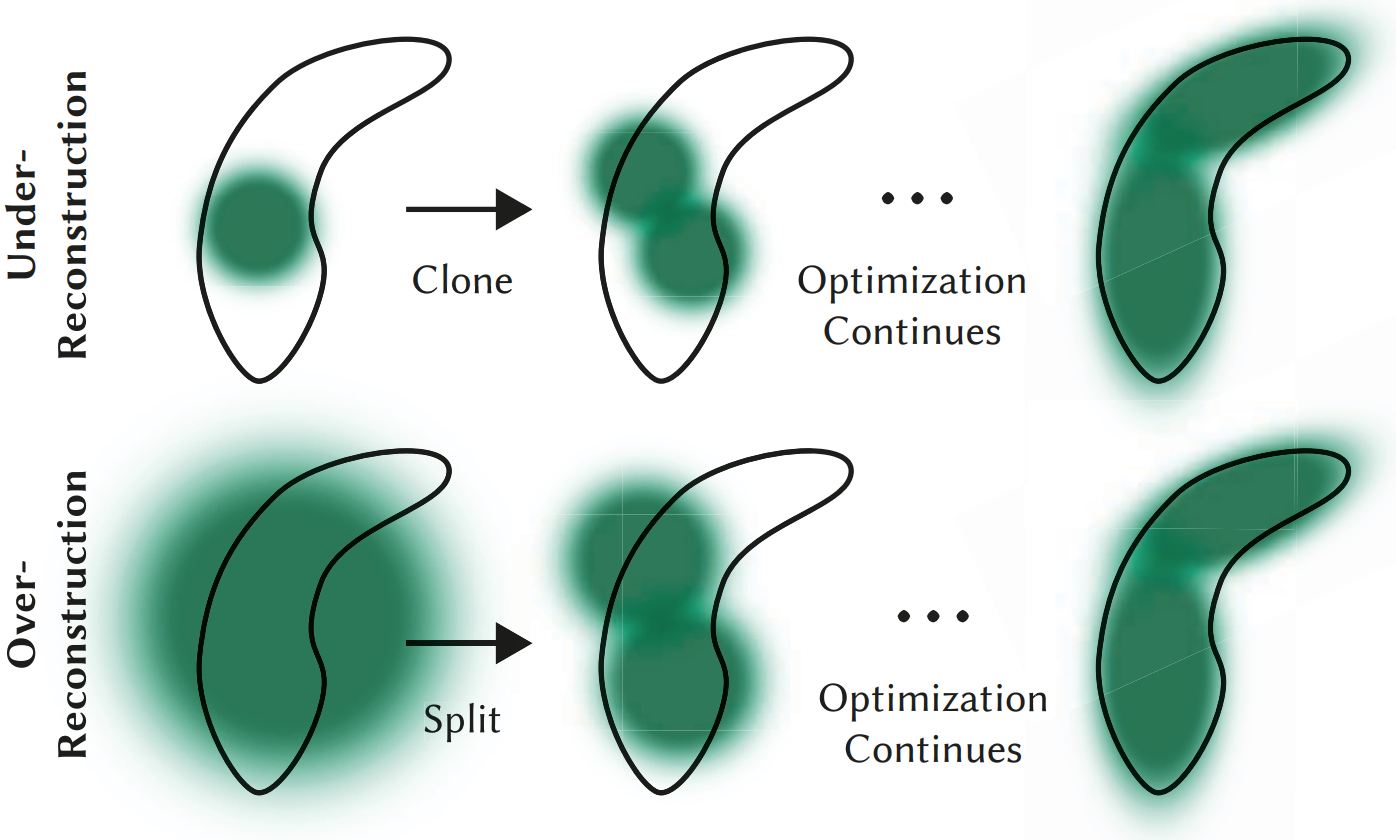
\includegraphics[width=0.5\linewidth]{3dgs-adaptive-densification.png}
		\smallskip
		\caption{Adaptive Density Control}
	\end{figure}
	\mode<presentation>{\blfootnote{\href{https://repo-sam.inria.fr/fungraph/3d-gaussian-splatting/}{(SIGGRAPH 2023, Best Paper) 3D gaussian splatting for real-time radiance field rendering}}}
\end{frame}
